\section{Results}\label{sec:results}

The background yields in the three jet categories are shown in Table~\ref{tab:bkg_yields} while the signal yields corresponding to a limited selection of mass points are shown in Table~\ref{tab:sig_yields}. The signal yields correspond to $C'=1$ and $BR_\mathrm{new} = 0$.

\begin{table}[h!]\begin{center}
\caption{Prefit yields for each backgorund process in the three analysis categories. The uncertainties are shown for the processes estimated from simulation.}\label{tab:bkg_yields}
\small{\begin{tabular}{
c| c | c | c } \hline
             background process           &         0 jets                                          &          1 jet                                         &        VBF                                           \\ \hline
      WW                &    501.93 +/-       0.00 (         0 \%)              &     198.72 +/-       0.00 (         0 \%)             &      4.54 +/-       0.00 (         0 \%)               \\
      ggWW                &     37.28 +/-       5.77 (        15 \%)              &      19.63 +/-       3.04 (        15 \%)             &      1.05 +/-       0.16 (        15 \%)               \\
      top                &    188.75 +/-       0.00 (         0 \%)              &     330.05 +/-       0.00 (         0 \%)             &     25.06 +/-       0.00 (         0 \%)               \\
      DY                &     33.24 +/-       0.00 (         0 \%)              &      12.99 +/-       0.00 (         0 \%)             &      0.28 +/-       0.00 (         0 \%)               \\
      Fake                &     64.21 +/-      19.26 (        30 \%)              &      31.69 +/-       9.51 (        30 \%)             &      2.10 +/-       0.63 (        30 \%)               \\
      Vg                &     26.62 +/-       0.72 (         3 \%)              &      14.18 +/-       0.38 (         3 \%)             &      0.64 +/-       0.02 (         3 \%)               \\
     VgS                &      4.44 +/-       1.12 (        25 \%)              &       3.39 +/-       0.85 (        25 \%)             &      0.14 +/-       0.04 (        25 \%)               \\
     VZ                &     13.51 +/-       0.76 (         6 \%)              &      11.67 +/-       0.66 (         6 \%)             &      0.28 +/-       0.02 (         6 \%)               \\
     VVV                &      0.01 +/-       0.00 (         3 \%)              &       0.02 +/-       0.00 (         3 \%)             &      0.00 +/-       0.00 (         3 \%)               \\   
 ggH                &      5.31 +/-       0.40 (         7 \%)              &       2.25 +/-       0.11 (         5 \%)             &      0.09 +/-       0.02 (        21 \%)               \\
 qqH                &      0.07 +/-       0.00 (         4 \%)              &       0.27 +/-       0.01 (         4 \%)             &      0.23 +/-       0.01 (         4 \%)               \\
  WH                &      0.54 +/-       0.03 (         6 \%)              &       0.48 +/-       0.03 (         6 \%)             &      0.01 +/-       0.00 (         6 \%)               \\
  ZH                &      0.09 +/-       0.01 (         6 \%)              &       0.07 +/-       0.00 (         6 \%)             &      0.00 +/-       0.00 (         6 \%)               \\   
 ggZH                &      0.02 +/-       0.01 (        40 \%)              &       0.03 +/-       0.01 (        40 \%)             &      0.01 +/-       0.00 (        40 \%)               \\
 H$\to\tau\tau$                &      0.50 +/-       0.05 (         9 \%)              &       0.43 +/-       0.04 (         9 \%)             &      0.04 +/-       0.00 (         9 \%)               \\
      
\hline                                                                                                                                       
    background          &    876.51 +/-      20.17 (         2\%)               &     625.90 +/-      10.05 (         2\%)              &     34.46 +/-       0.65 (         2\%)               \\
\hline
\end{tabular}
}
\end{center}

\end{table}


\begin{table}[h!]\begin{center}
\caption{Prefit signal yields for different mass hypothesis and for $C'=1$ and $BR_\mathrm{new} = 0$ in the three analysis categories. The errors correspond to the theoretical uncertainties in the signal estimation.}\label{tab:sig_yields}
\small{\begin{tabular}{
c | c | c | c } \hline
                 Mass (\GeV)                               &          0 jets                                         &          1 jet                
                                  &         VBF                                  \\ \hline

\hline   \multicolumn{4}{c}{ggH} \\              \hline
 200                        &      90.21 +/-       6.67 (         7 \%)             &      37.47 +/-       1.81 (         5 \%)     &       1.25 +/-       0.26 (        21 \%)      \\
 400                        &      66.35 +/-       4.90 (         7 \%)             &      32.65 +/-       1.57 (         5 \%)     &       2.04 +/-       0.42 (        21 \%)      \\
 600                        &      13.86 +/-       1.05 (         8 \%)             &       8.56 +/-       0.44 (         5 \%)     &       0.68 +/-       0.14 (        21 \%)      \\
 800                        &       3.20 +/-       0.25 (         8 \%)             &       2.32 +/-       0.13 (         6 \%)     &       0.22 +/-       0.05 (        21 \%)      \\
 1000                       &       0.88 +/-       0.07 (         8 \%)             &       0.70 +/-       0.04 (         6 \%)     &       0.07 +/-       0.02 (        21 \%)      \\

\hline   \multicolumn{4}{c}{qqH} \\  \hline
 200                        &       1.54 +/-       0.06 (         4 \%)             &       6.18 +/-       0.25 (         4 \%)     &       5.05 +/-       0.20 (         4 \%)      \\
 400                        &       0.91 +/-       0.04 (         4 \%)             &       3.42 +/-       0.14 (         4 \%)     &       3.19 +/-       0.13 (         4 \%)      \\
 600                        &       0.50 +/-       0.02 (         4 \%)             &       1.95 +/-       0.08 (         4 \%)     &       1.88 +/-       0.08 (         4 \%)      \\
 800                        &       0.33 +/-       0.01 (         4 \%)             &       1.21 +/-       0.05 (         4 \%)     &       1.16 +/-       0.05 (         4 \%)      \\
 1000                       &       0.22 +/-       0.01 (         4 \%)             &       0.79 +/-       0.03 (         4 \%)     &       0.69 +/-       0.03 (         4 \%)      \\

\hline
\end{tabular}
}
\end{center}

\end{table}


For every mass point from 200\GeV up to 1\TeV the significance (or p-value) and the 95\% CL upper exclusion limit are calculated for five $C'$ parameters: 0.1, 0.3, 0.5, 0.7 and 1.0. For the moment only $BR_\mathrm{new} = 1$ is considered.
The significance and the p-value are extracted using the ProfileLikelihood method embedded in the CMS Higgs \textit{combine} package. The upper exclusion limit on the signal strength is instead obtained using the Asymptotic method.
In Fig.~\ref{fig:significance} is shown the significance as a function of the mass for the three jet categories and in Fig.~\ref{fig:significance_comb} the combination of all the categories is reported for $C' = 1$.

The dip in the significance plot around 250\GeV is understood and it is due to the fact that the signal and background shapes at that mass are very similar and the fit is not able to discriminate between the two contributions.

\begin{figure}[htb]
\centering
\subfigure[0 jets]{
\includegraphics[width=0.45\textwidth]{Figs/Significance/significance_0jet_all.pdf}
}
\subfigure[1 jet]{
\includegraphics[width=0.45\textwidth]{Figs/Significance/significance_1jet_all.pdf}
}
\\
\subfigure[VBF]{
\includegraphics[width=0.45\textwidth]{Figs/Significance/significance_2jet_all.pdf}
}
\caption{
    Significance as a function of the mass for 0 jets, 1 jet and VBF categories.}
    \label{fig:significance}
\end{figure}

\begin{figure}[htb]
\centering
\includegraphics[width=0.7\textwidth]{Figs/Significance/significance_012jet_all.pdf}
\caption{
    Combined significance as a function of the mass.}
    \label{fig:significance}
\end{figure}

The exclusion limits at 95\% CL on the signal strength are shown in Fig.~\ref{fig:limit_mu} for the three jet categories separately and in Fig.~\ref{fig:limit_mu_comb} for the combination of the three categories. The results corresponding to $BR_\mathrm{new} = 1$ and different choises of the $C'$ parameter are shown.

\begin{figure}[htb]
\centering
\subfigure[0 jets]{
\includegraphics[width=0.45\textwidth]{Figs/Limits/limit_0jet_mu.pdf}
}
\subfigure[1 jet]{
\includegraphics[width=0.45\textwidth]{Figs/Limits/limit_1jet_mu.pdf}
}
\\
\subfigure[VBF]{
\includegraphics[width=0.45\textwidth]{Figs/Limits/limit_2jet_mu.pdf}
}
\caption{
    95\% CL exclusion limits on the signal strength as a function of the mass for 0 jets, 1 jet and VBF categories for $BR_\mathrm{new}=0$ and variuos choises of $C'$.}
    \label{fig:limit_mu}
\end{figure}

\begin{figure}[htb]
\centering
\includegraphics[width=0.7\textwidth]{Figs/Limits/limit_012jet_mu.pdf}
\caption{
    Combined 95\% CL exclusion limit on the signal strength as a function of the mass for $BR_\mathrm{new}=0$ and variuos choises of $C'$.}
    \label{fig:limit_mu_comb}
\end{figure}

The exclusion limits at 95\% CL on the production ggH and VBF cross section times branching fraction are shown in Fig.~\ref{fig:limit_xsec} for the three jet categories separately and in Fig.~\ref{fig:limit_xsec_comb} for the combination of the three categories. The limits are reported for $C'=1$ and $BR_\mathrm{new}=0$.

\begin{figure}[htb]
\centering
\subfigure[0 jets]{
\includegraphics[width=0.45\textwidth]{Figs/Limits/limit_0jet_xsec_c10brn00.pdf}
}
\subfigure[1 jet]{
\includegraphics[width=0.45\textwidth]{Figs/Limits/limit_1jet_xsec_c10brn00.pdf}
}
\\
\subfigure[VBF]{
\includegraphics[width=0.45\textwidth]{Figs/Limits/limit_2jet_xsec_c10brn00.pdf}
}
\caption{
    95\% CL exclusion limits on the production ggH and VBF cross section times branching fraction as a function of the mass for 0 jets, 1 jet and VBF categories. The limits correspond to $C'=1$ and are obtained using the 2015 data set.}
    \label{fig:limit_xsec}
\end{figure}

\begin{figure}[htb]
\centering
\includegraphics[width=0.7\textwidth]{Figs/Limits/limit_012jet_xsec_c10brn00.pdf}
\caption{
    Combined 95\% CL exclusion limit on the production ggH and VBF cross section times branching fraction as a function of the mass. The limit corresponds to $C'=1$ and are obtained using the 2015 data set.}
    \label{fig:limit_xsec_comb}
\end{figure}


The expected exclusion limits on the cross section times branching fraction for the three jet categories separately and for the combination using the 2016 data set are shown in Figs.~\ref{fig:limit_xsec_2016} and \ref{fig:limit_xsec_comb_2016} respectively.


\begin{figure}[htb]
\centering
\subfigure[0 jets]{
\includegraphics[width=0.45\textwidth]{Figs/Limits/2016/limit_xsec_0j_GSM.pdf}
}
\subfigure[1 jet]{
\includegraphics[width=0.45\textwidth]{Figs/Limits/2016/limit_xsec_1j_GSM.pdf}
}
\\
\subfigure[VBF]{
\includegraphics[width=0.45\textwidth]{Figs/Limits/2016/limit_xsec_2j_GSM.pdf}
}
\caption{
    95\% CL exclusion limits on the production ggH and VBF cross section times branching fraction as a function of the mass for 0 jets, 1 jet and VBF categories. The limits correspond to $C'=1$ and are obtained with the 2016 data set.}
    \label{fig:limit_xsec_2016}
\end{figure}

\begin{figure}[htb]
\centering
\includegraphics[width=0.7\textwidth]{Figs/Limits/2016/limit_xsec_012j_GSM.pdf}
\caption{
    Combined 95\% CL exclusion limit on the production ggH and VBF cross section times branching fraction as a function of the mass. The limit corresponds to $C'=1$ and are obtained using the 2016 data set.}
    \label{fig:limit_xsec_comb_2016}
\end{figure}






\clearpage
\subsection{Unblinding using 2015 data}

The \mt shapes after the unblinding using 2015 data are shown in Fig.~\ref{fig:shapes_unblinded}.

\begin{figure}[htb]
\centering
\subfigure[0 jets - \mt]{
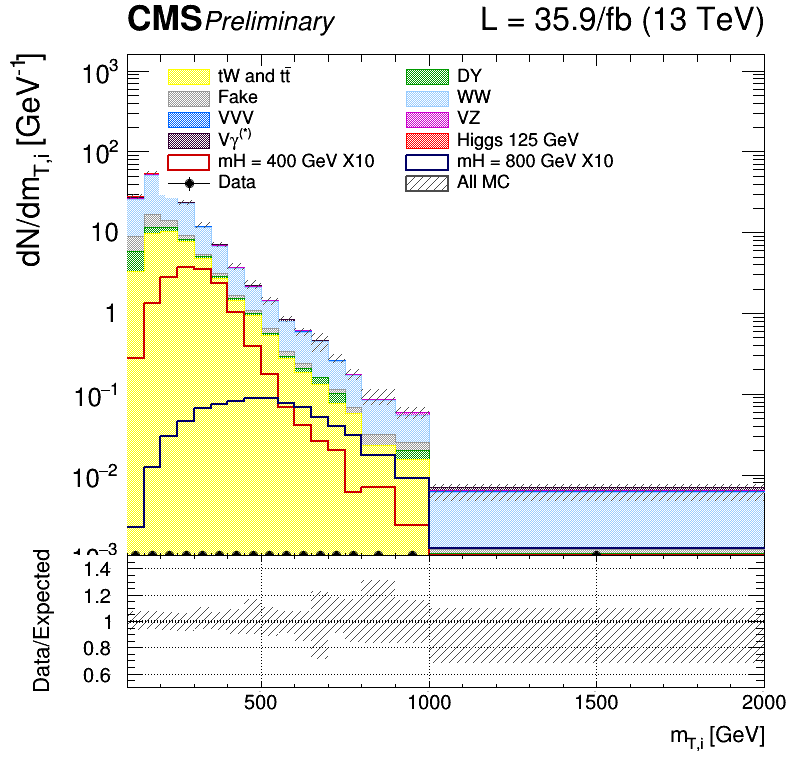
\includegraphics[width=0.45\textwidth]{Figs/Unblinding2015/log_cratio_hwwhm_13TeV_of_0j_mTi.png}
}
\subfigure[1 jet - \mt]{
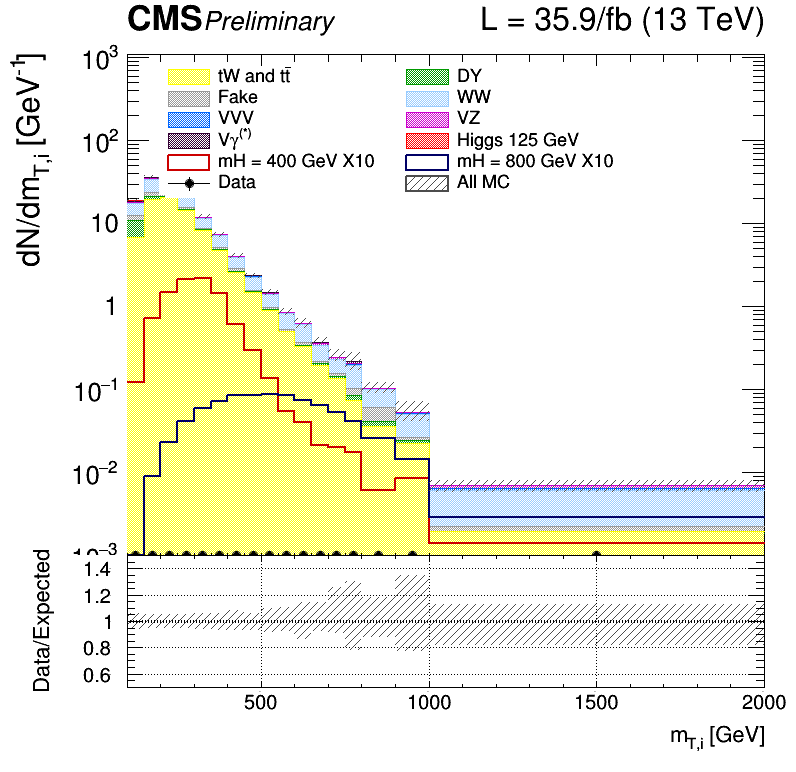
\includegraphics[width=0.45\textwidth]{Figs/Unblinding2015/log_cratio_hwwhm_13TeV_of_1j_mTi.png}
}
\\
\subfigure[VBF - \mt]{
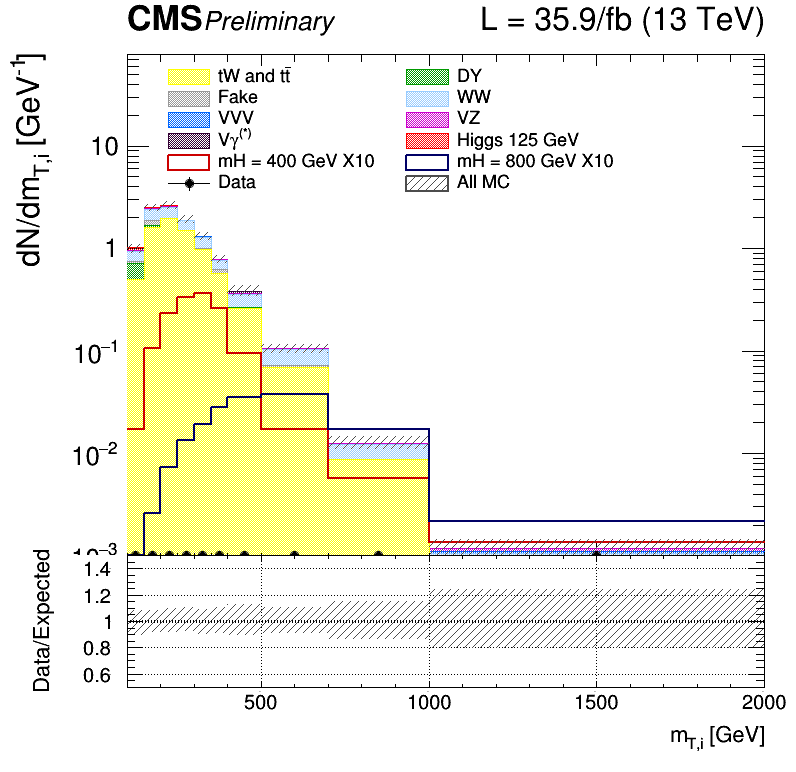
\includegraphics[width=0.45\textwidth]{Figs/Unblinding2015/log_cratio_hwwhm_13TeV_of_VBF_mTi_VBF.png}
}
\caption{
    Distributions of the \mt variable after the unblinding with 2015 data in the signal region for 0 jets, 1 jet and VBF categories. Two signal samples at $M_\mathrm{X} = 400$\GeV and 800\GeV are shown superimposed to the background pre-fit expectation.}
    \label{fig:shapes_unblinded}
\end{figure}

In Figs.~\ref{fig:limit_0j_unblind}, \ref{fig:limit_1j_unblind} and \ref{fig:limit_2j_unblind} are shown the exclusion limits on the cross section for the three jet categories separately, comparing two signal models with different widths, i.e. with $C' = 1.0$ and 0.5.


\begin{figure}[htb]
\centering
\subfigure[0 jets - $C'=0.5$]{
\includegraphics[width=0.45\textwidth]{Figs/Unblinding2015/limit_xsec_0jet_c05.pdf}
}
\subfigure[0 jets - $C'=1.0$]{
\includegraphics[width=0.45\textwidth]{Figs/Unblinding2015/limit_xsec_0jet_c10.pdf}
}
\caption{
   Expected and observed exclusion limits at 95\% CL on the production ggH and VBF cross section times branching fraction as a function of the mass for the 0 jets category. Two different hypothesis of the signal width are shown, corresponding to $C'=0.5$ ($\Gamma = 0.25\cdot\Gamma_\mathrm{SM}$) on the left plot and $C'=1.0$ ($\Gamma = \Gamma_\mathrm{SM}$) in the right plot.}
    \label{fig:limit_0j_unblind}
\end{figure}

\begin{figure}[htb]
\centering
\subfigure[1 jet - $C'=0.5$]{
\includegraphics[width=0.45\textwidth]{Figs/Unblinding2015/limit_xsec_1jet_c05.pdf}
}
\subfigure[1 jet - $C'=1.0$]{
\includegraphics[width=0.45\textwidth]{Figs/Unblinding2015/limit_xsec_1jet_c10.pdf}
}
\caption{
   Expected and observed exclusion limits at 95\% CL on the production ggH and VBF cross section times branching fraction as a function of the mass for the 1 jet category. Two different hypothesis of the signal width are shown, corresponding to $C'=0.5$ ($\Gamma = 0.25\cdot\Gamma_\mathrm{SM}$) on the left plot and $C'=1.0$ ($\Gamma = \Gamma_\mathrm{SM}$) in the right plot.}
    \label{fig:limit_1j_unblind}
\end{figure}

\begin{figure}[htb]
\centering
\subfigure[2 jets - $C'=0.5$]{
\includegraphics[width=0.45\textwidth]{Figs/Unblinding2015/limit_xsec_2jet_c05.pdf}
}
\subfigure[2 jets - $C'=1.0$]{
\includegraphics[width=0.45\textwidth]{Figs/Unblinding2015/limit_xsec_2jet_c10.pdf}
}
\caption{
   Expected and observed exclusion limits at 95\% CL on the production ggH and VBF cross section times branching fraction as a function of the mass for the VBF category. Two different hypothesis of the signal width are shown, corresponding to $C'=0.5$ ($\Gamma = 0.25\cdot\Gamma_\mathrm{SM}$) on the left plot and $C'=1.0$ ($\Gamma = \Gamma_\mathrm{SM}$) in the right plot.}
    \label{fig:limit_2j_unblind}
\end{figure}

The combined exclusion limit is shown in Fig.~\ref{fig:limit_comb_unblind}.

\begin{figure}[htb]
\centering
\subfigure[0+1+2 jets - $C'=0.5$]{
\includegraphics[width=0.45\textwidth]{Figs/Unblinding2015/limit_xsec_012jet_c05.pdf}
}
\subfigure[0+1+2 jets - $C'=1.0$]{
\includegraphics[width=0.45\textwidth]{Figs/Unblinding2015/limit_xsec_012jet_c10.pdf}
}
\caption{
   Expected and observed exclusion limits at 95\% CL on the production ggH and VBF cross section times branching fraction as a function of the mass combining the three jet categories. Two different hypothesis of the signal width are shown, corresponding to $C'=0.5$ ($\Gamma = 0.25\cdot\Gamma_\mathrm{SM}$) on the left plot and $C'=1.0$ ($\Gamma = \Gamma_\mathrm{SM}$) in the right plot.}
    \label{fig:limit_comb_unblind}
\end{figure}


\clearpage
\subsection{Unblinding using 2016 data}
